\shorthandoff{"}
\chapter{Methodik}
\label{ch:methodik}

\section{Art der Forschung}
\label{ch:methodik:art}
Um die Forschungsfrage dieser Master-Thesis zu beantworten, wird eine quantitative Forschungsarbeit in Form eines Experiments durchgeführt. In diesem Kontext werden für einen A/B-Test zwei Versionen eines Empfehlungssystems zur Besetzung offener Projektpositionen entwickelt. Eine der beiden Anwendungen verfolgt einen unilateralen, die andere einen bilateralen Ansatz. Beide Empfehlungssysteme erhalten als Eingabe dieselben offenen Projektpositionen. Für diese Stellen sortieren die Anwendungen die vorhandenen Mitarbeiter eines Betriebs und geben diese in Form einer Liste zurück.

Die Ausgaben beider Systeme werden Projektmanagern vorgelegt. Diese bewerten für jede Liste auf einer vordefinierten Skala, welche Arbeitsleistung sie von denen in der vorliegenden Reihenfolge dargestellten Mitarbeitern erwarten. Dabei wird evaluiert, ob sie die erwartete Leistung der vorgeschlagenen Angestellten des bilateralen Empfehlungssystems höher bewerten, als die der unilateralen Variante.

Die Angestellten des Unternehmens erhalten die Beschreibungen der offenen Projektpositionen. Daraufhin bewerten sie auf einer vordefinierten Skala, wie zufrieden sie voraussichtlich mit der Tätigkeit auf den vorliegenden Projektpositionen sein werden. Hierbei wird für beide Empfehlungssysteme überprüft, ob eine hohe erwartete Zufriedenheit der Angestellten mit einer hohen Positionierung in den Ergebnislisten korreliert.

Abschließend werden die Bewertungen von Projektmanagern und Angestellten hinsichtlich der Ergebnisse der beiden Empfehlungssysteme verglichen. Hierbei wird bestimmt, ob die bilaterale Recommender Engine im direkten Vergleich mit dem unilateralen Ansatz sowohl auf Seiten der Projektmanager für eine höhere erwartete Leistung als auch aus Perspektive der Mitarbeiter für eine höhere erwartete Zufriedenheit sorgte.

\section{Versuchsaufbau}
\label{ch:methodik:versuchsaufbau}
Durchgeführt wird das Experiment mit Projektmanagern und Mitarbeitern der EXXETA AG mit Hauptsitz in Karlsruhe. Das Unternehmen ist spezialisiert auf IT-Beratungsleistungen und arbeitet vorrangig projektbasiert. Passende Angestellte zu offenen Projektpositionen zuzuordnen ist in diesem Betrieb dementsprechend eine häufig auftretende Aufgabe. Daher liegen Informationen über die Kompetenzen der Mitarbeiter bereits in einer strukturieren Form vor.

Die Mitarbeiter der EXXETA AG pflegen ihre Kompetenzen in einem Intranet. Dort steht eine Liste mit 551 Fähigkeiten wie beispielsweise "Java", "DSGVO" und "Digitale Transformation" zur Verfügung. Diese können die Angestellten über die in Abbildung \ref{fig:methodik:versuchsaufbau:daten:abb1} dargestellte Skala bewerten.

\begin{figure}[h]
	\centering
	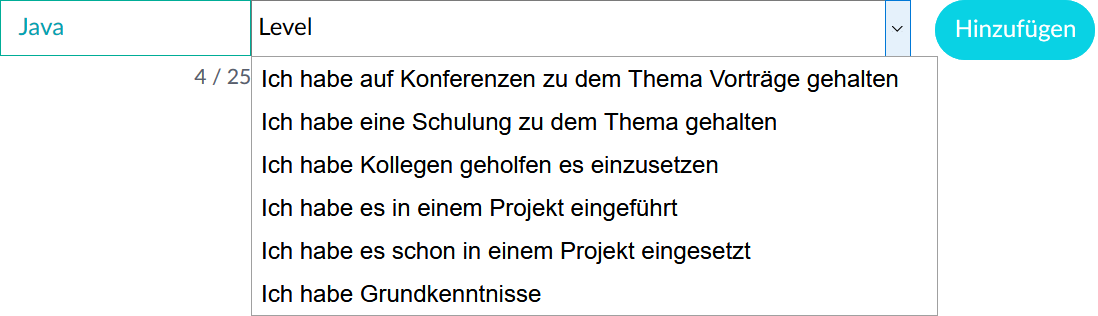
\includegraphics[width=1\textwidth]{gfx/skill-level.png}
	\caption{Hinzufügen einer Fähigkeit mit Angabe des entsprechenden Kenntnisniveaus im EXXETA-Intranet}
	\label{fig:methodik:versuchsaufbau:daten:abb1}
\end{figure}

Die in Abbildung \ref{fig:methodik:versuchsaufbau:daten:abb1} dargestellten Abstufungen werden beim Speichern in ganzzahlige Werte von null ("Ich habe Grundkenntnisse") bis sechs ("Ich habe auf Konferenzen zu dem Thema Vorträge gehalten") übertragen.

Aufgrund der klaren Beschreibungen der einzelnen Stufen in Abbildung \ref{fig:methodik:versuchsaufbau:daten:abb1} kann Bias bei der Selbsteinschätzung weitgehend ausgeschlossen werden. Außerdem ist es in der vorliegenden Problemstellung gut möglich, dass einzelne Mitarbeiter ihre Kompetenzen bewusst besser oder schlechter einschätzen als andere Kollegen. Dieser Sachverhalt kann insbesondere auf längere Berufserfahrung zurückgeführt werden. Daher wird bei der Empfehlungsbestimmung auf eine Mittelwert-Zentrierung verzichtet.

Die Kompetenzen der Mitarbeiter und die zugehörigen Bewertungen dienen im Experiment als Eingabe für einen grundlegenden Algorithmus, welcher sowohl für das unilaterale als auch das bilaterale Empfehlungssystem gleich ist.

\subsection{Grundlegender Algorithmus}
\label{ch:methodik:versuchsaufbau:grundlegend}
Um Mitarbeiter für offene Projektpositionen vorzuschlagen, wird zunächst die Katz-Zentralität angewendet. Dieser speicherbasierte Graphenalgorithmus wurde in Kapitel \ref{ch:empfehlungssysteme:cf:speicherbasiert} vorgestellt. Ein Nutzen dieses Ansatzes ist die zuverlässige Lösung des Sparsity Problems. Vorteilhaft gegenüber modellbasierten Methoden ist außerdem die Langlebigkeit des Verfahrens. Sollten sich nach Durchführung des Experiments Daten im Unternehmen signifikant verändern oder neue Kompetenzen im Intranet hinzugefügt werden, ist der speicherbasierte Ansatz weiterhin unverändert anwendbar. Die dabei zu erwartende hohe Komplexität ist in der vorliegenden Problemstellung tolerierbar, da sich zum Zeitpunkt des Experiments unter 1.000 Mitarbeiter im Unternehmen befinden.

Um neben dem Sparsity Problem auch den Kaltstart zu beheben, werden zusätzlich zu den Fähigkeiten der Mitarbeiter auch deren Teamzuordnungen in Form eines hybriden Ansatzes beachtet. Bei der EXXETA AG arbeiten stets Mitarbeiter in einem Team, welche ähnliche Kompetenzen beherrschen. Deren Manager ist eine fachliche Führungskraft, dessen Fähigkeiten weitgehend repräsentativ für sein Team sind. Seine Kompetenzen sind jedoch in der Regel stärker ausgeprägt.

Die Bewertungen der Fähigkeiten und die Teamzuordnungen können für alle Mitarbeiter der EXXETA AG über eine \acsu{REST}-Schnittstelle in Form von \acsu{JSON} aus dem Intranet abgefragt werden. Wäre John Doe aus Tabelle \ref{tbl:empfehlungssysteme:arbeitsweise:tbl1} ein Mitarbeiter der EXXETA AG, würden seine zurückgegebenen Daten dem folgenden Quellcode \ref{qc:methodik:versuchsaufbau:daten:qc1} entsprechen.

%\begin{minipage}{\linewidth}
\lstinputlisting[
language=json,
caption=Beispiel für ein Mitarbeiter-\acsu{JSON} der \acsu{REST}-Schnittstelle des Intranets der EXXETA AG (Auszug),
captionpos=b,
label=qc:methodik:versuchsaufbau:daten:qc1
]{gfx/john.json}
%\end{minipage}

In Quellcode \ref{qc:methodik:versuchsaufbau:daten:qc1} ist zu erkennen, dass die Bewertungen in Tabelle \ref{tbl:empfehlungssysteme:arbeitsweise:tbl1} um eins höher sind, als die Beurteilungen im zurückgegebenen \ac{JSON}. Damit ein Kantengewicht von null ausschließlich nicht vergebene Einschätzungen symbolisiert, werden die Bewertungen des \acp{JSON} vor der Empfehlungsberechnung um eins erhöht.

Um Rechenleistung einzusparen, werden die Teams nicht als zusätzliche Knoten in den Graphen eingefügt. Die Beziehungen werden stattdessen über direkte Kanten zwischen Kollegen dargestellt. Das Kantengewicht zwischen zwei Teammitgliedern beträgt dabei eins und das Gewicht von einem Angestellten zu seinem Manager zwei. Über diesen Ansatz sind alle Teammitglieder schwach miteinander verbunden, sodass auch im Fall eines Kaltstarts für Mitarbeiter ohne explizite Bewertungen aussagekräftige Beurteilungen bestimmt werden können. Außerdem erhalten die Teammanager durch das höhere Kantengewicht eine stärkere Zentralität im Graphen.  Daher profitieren sämtliche Teammitglieder transitiv von den repräsentativen Fähigkeiten ihres Managers.

Um Empfehlungen erhalten zu können, muss ein Projektmanager die für eine offene Projektposition relevanten Fähigkeiten mitsamt der benötigten Kompetenzniveaus festlegen. Diese Daten werden, wie in Kapitel \ref{ch:empfehlungssysteme:cf:speicherbasiert} im Kontext der Gruppen-Recommender Engines beschrieben, in Form eines Pseudo-Mitarbeiters ebenfalls in den Graphen eingefügt.

Abbildung \ref{fig:methodik:versuchsaufbau:unilateral:abb1} zeigt die Darstellung der Kompetenzen und die Teamzuordnungen der Angestellten aus Tabelle \ref{tbl:empfehlungssysteme:arbeitsweise:tbl1} in der Form eines Graphen. Außerdem wurde eine offene Projektposition in Form eines Pseudo-Mitarbeiters eingefügt. In der Grafik wird Jane Doe als Team-Managerin betrachtet.

\begin{figure}[h]
	\centering	
	\begin{tikzpicture}[node distance={32mm}, thick, main/.style = {draw, circle}] 
		\node[main, fill=itemcolor] (MongoDB) {$MongoDB$}; 
		\node[main, fill=itemcolor] (Python) [below right of=MongoDB] {$Python$}; 
		\node[main, fill=itemcolor] (MySQL) [above right of=Python] {$MySQL$}; 
		\node[main, fill=itemcolor] (Java) [below right of=MySQL] {$Java$}; 
		\node[main, fill=itemcolor] (HDFS) [above right of=Java] {$HDFS$}; 
		\node[main, fill=itemcolor] (Spark) [below right of=HDFS] {$Spark$};
		
		\node[main, fill=usercolor] (Jane) [above right of=MongoDB] {$Jane D.$}; 
		\node[main, fill=usercolor] (John) [above left of=HDFS] {$John D.$}; 
		\node[main, fill=usercolor] (Max) [below of=MySQL] {$Max M.$};
		\node[main, fill=usercolor] (Erika) [above right of=HDFS] {$Erika M.$};
		\node[main, fill=usercolor] (Projekt) [below of=Java] {$Projekt$}; 
		
		\draw (Jane) -- node[midway, right] {4} (Python);
		\draw (Jane) -- node[midway, above] {3} (MySQL);
		\draw (Jane) -- node[midway, above] {3} (MongoDB);
		
		\draw (John) -- node[midway, right] {1} (HDFS);		
		\draw (John) -- node[midway, right] {3} (Java);
		\draw (John) -- node[midway, above] {2} (MySQL);
		
		\draw (Erika) -- node[midway, above] {5} (HDFS);
		\draw (Erika) -- node[midway, right] {3} (Spark);
		
		\draw (Max) -- node[midway, above] {2} (Java);
		\draw (Max) -- node[midway, above] {3} (Python);
		\draw (Max) -- node[midway, right] {1} (MySQL);
		
		\draw (Jane) -- node[midway, above] {2} (John);
		\draw (Jane) -- node[midway, left] {2} (Max);
		\path (Jane) edge[bend left=25] node[midway, above] {2} (Erika);
		
		\draw (John) -- node[midway, right] {1} (Max);
		\draw (John) -- node[midway, above] {1} (Erika);
		
		\path (Max) edge[bend right=40] node[midway, above] {1} (Erika);
		
		%\draw (Projekt) -- node[midway, above] {4} (Java);
		%\draw (Projekt) -- node[midway, above] {2} (HDFS);
		%\draw (Projekt) -- node[midway, above] {3} (Spark);
		\path (Projekt) edge[bend left=40] node[midway, above] {3} (MongoDB);
		\path (Projekt) edge[bend left=25] node[midway, above] {4} (Python);
		\path (Projekt) edge[bend right=25] node[midway, above] {3} (Spark);
	\end{tikzpicture}
	
	\caption{Graph aus Abbildung \ref{fig:empfehlungssysteme:cf:speicherbasiert:abb2} mit zusätzlicher Teamzuordnung und offener Projektposition}
	\label{fig:methodik:versuchsaufbau:unilateral:abb1}
\end{figure}

Anhand der Daten des Graphen folgt die Bestimmung der Katz-Zentralität. Für die Beispieldaten aus Abbildung \ref{fig:methodik:versuchsaufbau:unilateral:abb1} ergibt sich mit $\beta = 0.1$ die folgende Matrix \ref{frml:methodik:versuchsaufbau:unilateral:formel1}. Die vollständige Berechnung kann in Anhang \ref{ch:nebenrechnungen:katzZentralitaetPseudoMitarbeiter} nachvollzogen werden.

\begin{gather}
	\begin{bmatrix}
		77.19 & 43.00 & 47.69 & 52.75 & 45.71 & 23.45 & 65.39 & 37.33 & 37.17 & 28.15 & 28.02\\
		43.00 & 23.94 & 26.58 & 29.33 & 25.25 & 13.35 & 36.10 & 20.82 & 20.47 & 15.79 & 15.55\\
		47.69 & 26.58 & 29.77 & 32.48 & 28.17 & 14.47 & 40.09 & 22.87 & 22.76 & 18.04 & 17.68\\
		52.75 & 29.33 & 32.48 & 35.89 & 31.12 & 16.18 & 44.61 & 25.38 & 25.16 & 19.17 & 19.08\\
		45.71 & 25.25 & 28.17 & 31.12 & 27.33 & 13.80 & 38.95 & 21.87 & 22.21 & 16.61 & 16.95\\
		23.45 & 13.35 & 14.47 & 16.18 & 13.80 & 7.24 & 19.75 & 11.32 & 11.17 & 8.57 & 8.48\\
		65.39 & 36.10 & 40.09 & 44.61 & 38.95 & 19.75 & 55.12 & 31.30 & 31.30 & 23.65 & 23.71\\
		37.33 & 20.82 & 22.87 & 25.38 & 21.87 & 11.32 & 31.30 & 17.90 & 17.76 & 13.52 & 13.42\\
		37.17 & 20.47 & 22.76 & 25.16 & 22.21 & 11.17 & 31.30 & 17.76 & 17.82 & 13.43 & 13.49\\
		28.15 & 15.79 & 18.04 & 19.17 & 16.61 & 8.57 & 23.65 & 13.52 & 13.43 & 10.60 & 10.40\\
		28.02 & 15.55 & 17.68 & 19.08 & 16.95 & 8.48 & 23.71 & 13.42 & 13.49 & 10.40 & 10.39
	\end{bmatrix}
	\label{frml:methodik:versuchsaufbau:unilateral:formel1}
\end{gather}

Diese entstehende Matrix \ref{frml:methodik:versuchsaufbau:unilateral:formel1} dient als Eingabe für die unilaterale und die bilaterale Empfehlungs-Komponente. Beide Module unterscheiden sich, wie bei einem A/B-Test gefordert, ausschließlich in der Art, über welche sie die Ergebnisse des Katz-Algorithmus sortieren.

\subsection{Unilaterale Empfehlungs-Komponente}
\label{ch:methodik:versuchsaufbau:unilateral}
Anschließend wird für jede vom Projektmanager geforderte Kompetenz die absolute Differenz zwischen Pseudomitarbeiter und allen anderen Angestellten bestimmt. Im letzten Schritt werden die Mitarbeiter nach geringster Abweichung sortiert und an den Projektmanager zurückgegeben.

\subsection{Bilaterale Empfehlungs-Komponente}
\label{ch:methodik:versuchsaufbau:bilateral}

\newpage
Zu erhebende Daten:\\
- Für jeden Mitarbeiter erheben: Wichtigkeit (true/false) --> Auch für Dinge, die man noch nicht kann\\
- Für jeden Mitarbeiter erheben: Welche Auswirkung hat es, wenn im Projekt nicht ausgelastet (Kurve A bis C) --> Alle drei Antwortmöglichkeiten positiv formulieren --> z.B. Freiräume nutzen

Erstellen des Graphen:\\
- Aus Skills (kollaboratives Filtern) und Teamzuordnung (Inhaltsbasiertes Filtern) einen tripartiten Graphen erstellen\\

Eingabe der offenen Projektposition:\\
- Benötigt: Fähigkeiten und Wichtigkeit (Boolean)

Algorithmus:\\
- Berechnung der Katz-Zentralität\\
- Für jeden relevanten Mitarbeiter auf Basis von Abbildung \ref{fig:methodik:abb2} den finalen Wert bestimmen --> Hierbei je nach Wichtigkeit die Kurve stauchen --> Wenn für Projektmanger wichtig, die durchgezogene Linie doppelt so steil; Wenn für Mitarbeiter wichtig, rechte Seite doppelt so steil; Auswahl der Kurve anhand der Information des Mitarbeiters\\
- Summe für alle Fähigkeiten eines Projektes für jeden Mitarbeiter berechnen

\begin{figure}[h]
	\centering
	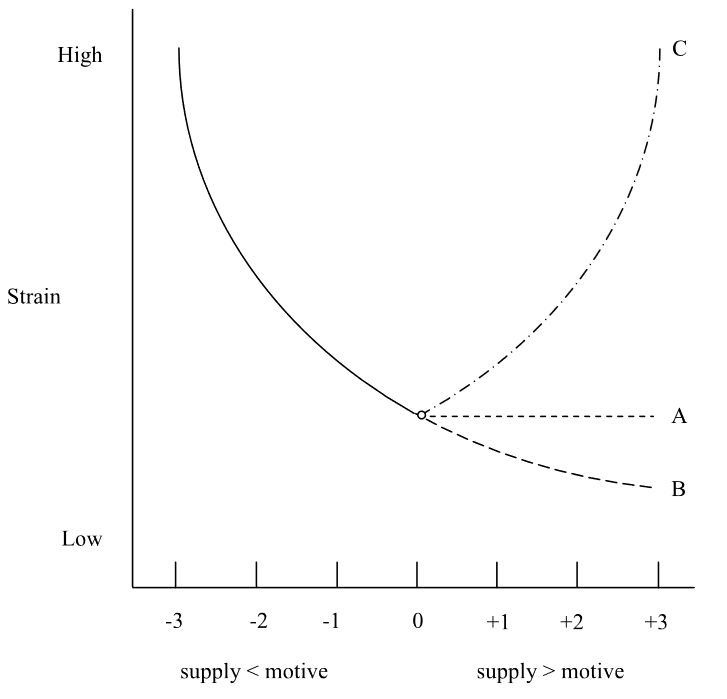
\includegraphics[width=0.75\textwidth]{gfx/ueberschuss_supply_motive.png}
	\caption{Auswirkungen eines Bedürfnisse-Angebote Misfits \cite[S. 23]{edwards:2008}\\(Bearbeitet von \myName)}
	\label{fig:methodik:abb2}
\end{figure}

- Algorithmus einmal durchführen mit Wichtigkeiten und einmal ohne (bilateral vs. unilateral)\\
- Ausgabe der sortierten Liste (mit allen Mitarbeitern (zB 25))\\
- Eingabe der Projektposition und Algorithmus für jede Projektposition wiederholen

\section{Evaluation}
\label{ch:methodik:evaluation}
Evaluation für Projektmanager:\\
- Erhält für jedes Projekt beide Listen und gibt auf einer Skala von 1 bis 5 an, wie hoch der die Leistung der empfohlenen Mitarbeiter in diesem Projekt einschätzen würde

Evaluation für Mitarbeiter:\\
- Jeder Mitarbeiter muss für jedes Projekt auf einer Skala von 1 bis 5 bewerten, wie zufrieden er wäre, wenn er darin arbeiten würde\\
- Ergebnisliste wird in Intervalle geteilt --> z.B. Zufriedenheit 5 bedeutet bei 25 Teilnehmern, dass der Nutzer im ersten Intervall sein muss --> Abweichung bestimmen --> Je weniger Abweichung, desto besser --> Durchschnittliche Abweichung von unilateral und bilateral vergleichen
\shorthandon{"}
